\section{Review of the Macroeconometric Literature}\label{sec:empirical_review}


It worth noting that most papers that includes residential investment has failed to treat it macroeconomically, restricting it to microeconomic and regional issues (\cite{arestis_u.s._2008}).
However, after the burst of the US housing bubble, there have been a growing attention in the macroeconomic implications of residential investment.
In this context, we analyze the macroeconometric literature that explicitly includes housing to evaluate the determinants of its growth rate.
Each model will be analyzed according to the compatibility with demand-led growth agenda as well as the possibility of including asset bubbles.

In this sense, \textcite{poterba_tax_1984} contribution stands out once it does not assume instantly convergence of real estate supply to the desired level.
Furthermore, this theoretical frame considers residential investment as induced positively by house prices.
Despite the novelty, this work does not include asset bubbles.
In this context,  \textcite{arestis_residential_2015} update \textcite{poterba_tax_1984} framework by estimating an autoregressive distributed lag (ARDL) model for 17 OECD countries.
In summary, they conclude that residential investment depends mainly on disposable income.
This result would  question the possibility of treating housing as an autonomous expenditure and jeopardize the analysis from the Sraffian supermultiplier perspective.
However, the authors themselves find that this result is not statistically significant for the US in which real house prices and the volume of banking credit are the main determinant of residential investment.
In this sense, this result allows considering housing as a non-capacity creating autonomous expenditure.

Alternatively, \textcite{huang_is_2018} assess both \textcite{leamer_housing_2007} hypotheses related to residential investment (prediction and causality). 
To do so, they estimate a Structural Vector Autoregressive (SVEC) model with wavelets transformation for some OECD countries
They find residential investment is not only as monetary policy transmission channel, but it also has temporally distinct effects on business cycle.
In the short-run, housing is more predictive while house prices have a bigger influence in the long-run\footnote{
	More precisely, \textcite{huang_is_2018} also conclude that residential investment prediction increases with its share on GDP.
}. 
These distinct temporal influence of housing occurs due to the large wealth effect in the long-run while credit and collateral effect are more relevant in the short-run.
Regarding the causal relationship described by \textcite{leamer_housing_2007}, 
\textcite{huang_is_2018} report inconclusive results for all countries due to their institutional heterogeneity\footnote{
	However, \textcite{huang_is_2018} claim that for most G7 countries, residential investment at least amplify the business cycle.
}, but remains valid for the US.
Despite the inconclusive results on fluctuations, they find that the variables associated with residential investment (house prices, real mortgage rate --- deflated by a general price index --- and bank spread) lead the business cycle.

Despite clarifying some macroeconomics  implications of housing on the business cycle, the results reported above are centered on supply side variables.
\textcite{gauger_residential_2003}, on the other hand, evaluate the consequences of deregulation of depository institutions throughout the 1980s.
To do so, they estimate a VECM between monetary aggregates (M2), GDP, residential investment and alternate between short-term government bonds and long-term mortgage interest rates. 
They report an increasing contribution of long-term mortgages interest rate over resident investment variance after those institutional chances mentioned above:

\begin{quotation}
	The findings for the two interest rates give valuable information to evaluate results in other studies. Results here suggest that use of a short-term FFR and post-deregulation data may lead to conclusions that `interest rate shocks are much less important after deregulation.' The fuller state of evidence here indicates that interest rate shocks remain important post-deregulation; however, now it is the long-term rate shocks that carry more information for housing sector movements (\cite[p.~346]{gauger_residential_2003})
\end{quotation}
It worth noting that \textcite{gauger_residential_2003} work reports other two interesting results:
	(i) GDP level is determined --- as Sraffian supermultiplier  suggests --- by residential investment and both expenditures share a common long-term trend;
	(ii) show some relevant institutional changes in real estate market.

Figure \ref{Fig:CreditFDICIA} illustrates item (ii) mentioned above in which we mark some reforms that occurred due to the savings and loans crisis throughout the 80's and early 90's.
This institutional changes --- notably Financial Institutions Reform, Recovery, and Enforcement Act (FIRREA) in 1989 and Federal Deposit Insurance Corporation Improvement Act  (FDICIA) in 1991 --- increased the credit volume to households\footnote{
	\textcite{federal_deposit_insurance_corporation_savings_1997} argues that this consequence stems from the different regulation of S\&L compared to commercial banks. The financial deregulation of the 1980s encouraged speculation in other sectors, especially real estate. As a consequence, engendered a banking run, increasing overall credit volume, which, however, was followed by the S\&L crisis:
	\begin{quotation}
		Clearly, competition from savings and loans did not cause the various crises experienced by the commercial banking industry during the 1980s; these crises would have occurred regardless of the thrift situation. But the channeling of large volumes of deposits into high-risk institutions that speculated in real estate development did create marketplace distortions (\cite[p.~168]{federal_deposit_insurance_corporation_savings_1997})
	\end{quotation}
	Therefore, the increase in credit volume cannot be dissociated from speculation with real estate.
}\footnote{
	According to \textcite{federal_deposit_insurance_corporation_savings_1997}, had two main objectives:
		(i) Recapitalize the bank insurance fund and;
		(ii) Reform the deposit guarantee system and bank regulation to minimize  taxpayer in the event of bank collapse (\cite{mishkin_evaluating_1997}).
		\textcite[p.~170]{federal_deposit_insurance_corporation_savings_1997} describe banking operation before FDICIA as follows:
		\begin{quotation}
			Legislation for S\&Ls was driven by the public policy goal of encouraging home ownership. It began with the Federal Home Loan Bank Act of 1932, which established the Federal Home Loan Bank System as a source of liquidity and low-cost financing for S\&Ls.
		\end{quotation}
	and the implications after its implementation is depicted as:
		\begin{quotation}
			Prior to the act’s passage, the FDIC and the Federal Savings and Loan Insurance Corporation provided 100 percent \textit{de facto} deposit insurance at almost all failed banks. The FDIC did so by comparing bids to acquire the entire bank (including all its deposits) with the cost of liquidating the bank, which generally produced the result that covering all deposits was less expensive (FDIC 2003, chap. 2). FDICIA sought to change this process by mandating least-cost resolution, which required consideration of all possible resolution methods (FDIC 2003, chap. 2) (\cite[p.~iii]{wall_too_2010})
		\end{quotation}
		
}. As a consequence, real estate finance has increased considerably in the following periods.

\begin{figure}[htb]
	\centering
	\caption{Mortgage and Consumer credit growth rate (1979-2019)}
	\label{Fig:CreditFDICIA}
	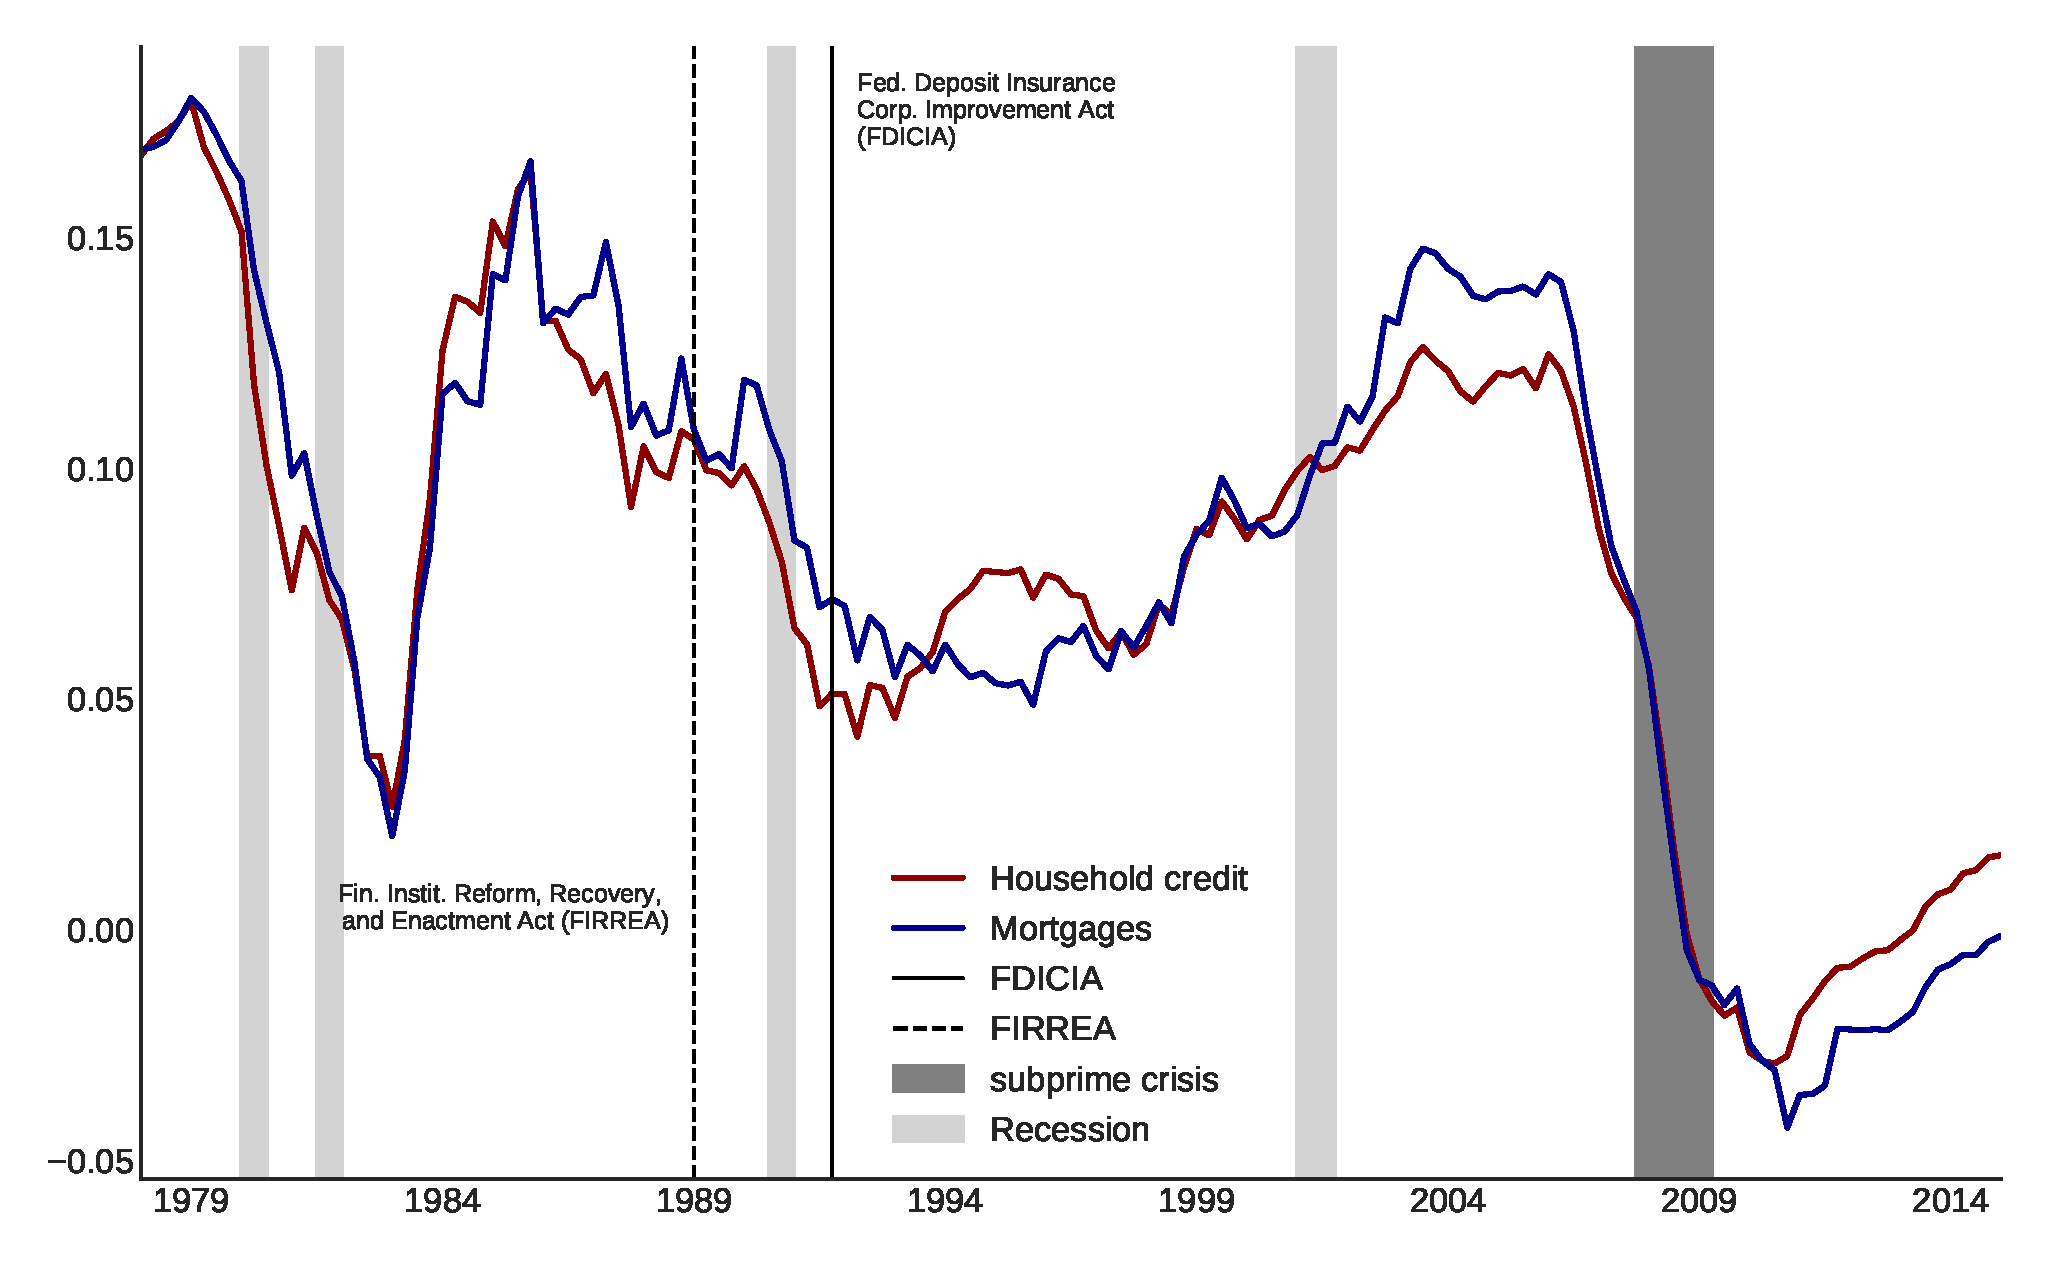
\includegraphics[width=\textwidth]{./figs/FDICIA.eps}
	\caption*{\textbf{Source:} U.S. Bureau of Economic Analisys, Authors' elaboration}
\end{figure}
Although \textcite{gauger_residential_2003} emphasize the relevance of long-term mortgages interest rate in residential investment dynamics, this procedure is not appropriate once policy rate is determined by monetary aggregates.
Thus, such a proposal is incompatible with modern macroeconomic theory in which policy rate is an exogenous variable determined through a decision-making process (\cite[p.~230--256]{lavoie_post-keynesian_2015}).

One way to include residential investment in demand-led growth agenda without incurring problems mentioned above is the houses' own interest rate proposed by \textcite{teixeira_crescimento_2015}.
In summary, this particular real interest rate depicts both debt service and capital gains effects in households' net worth.
On the following section, we discuss this proposal in further details and then evaluate its relevance in a macroeconometric model.

